\subsubsection{Justificación}

Actualmente casi todos contamos con computadores con una capacidad respetable en comparación a las últimas tecnologías existentes,
pero estamos descuidando un área muy popular, los cuales son los sistemas embebidos.

Es por eso que en nuestro trabajo hemos optado por trabajar con un equipo con arquitectura ARM\footnote{http://es.wikipedia.org/wiki/ARM},
pues su capacidad de procesamiento es mucho menor, pero aspira alcanzar procesamientos al mismo nivel que un computador normal.
Si nos damos cuenta, la mayoría de los dispositivos como celulares, pocketpc, netbooks, etc, poseen poca memoria y necesitan que cada operación que se realice
sobre ella sea lo más óptima posible.

Finalmente,
una mejora en un algoritmo en un computador de escritorio o notebook actual, quizás no podremos notar la diferencia,
pero en sistemas embebidos pueden significar un gran ahorro de tiempo y provocar un mayor desempeño.

\subsubsection{Hardware}

	El kit de desarrollo Intrinsyc's Cerf$^{TM}$Board 250 provee una plataforma 
flexible, con hardware y software de alto desempe\~no para desarrollar aplicaciones 
embebidas en forma r\'apida. El kit incluye:

\begin{itemize}
	\item Intel PXA250 (XScale)
	\item Tarjeta de expansi\'on Cerf IO 250
	\item Tarjeta de expansi\'on CerfComm 250
	\item Intrinsyc's I-Linux con kernel 2.4
\end{itemize}

\begin{center}
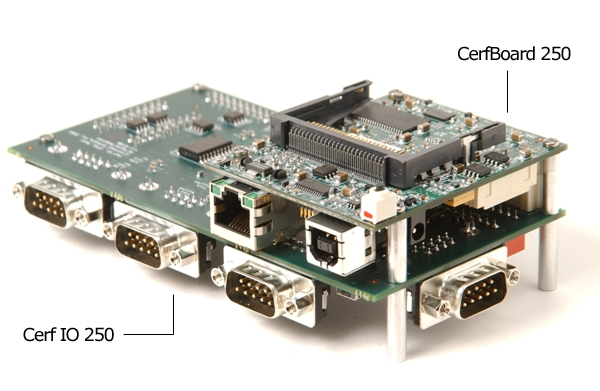
\includegraphics[scale=0.3]{images/board}
\end{center}

\subsubsection{Intel PXA250 (XScale)}

	El Intel PXA250 es un microprocesador basado en un n\'ucleo Intel XScale.
Intel XScale es una micro arquitectura RISC de 32-bit basado en una arquitectura ARM. Dise\~nado para un alto desempe\~no a costa de usar poca energ\'ia. Incorpora un conjunto completo de sistemas y perif\'ericos, funciones que le permite ser utilizado en una variedad de port\'atiles de mano.

	Posee las siguientes caracter\'isticas t\'ecnicas:

\begin{itemize}
	\item Frecuencia de 400MHz
	\item Memoria Principal de 64MB
	\item Cach\'e de instrucciones de 32KB
	\item Cach\'e de datos de 32KB
	\item B\'ufer de 256 bit
	\item Controlador de memoria basado en una arquitectura de memoria unificada, donde todos los dispositivos de memoria externos comparten un bus de direcci\'on y datos en com\'un.
	\item El controlador de memoria consiste en cuatro unidades de control principal para dar interfaz a memorias din\'amicas (SDRAM), memorias est\'aticas (ROM, SRAM, Flash), PCMCIA y chips similares.
	\item La memoria externa es vista como una colecci\'on lineal de bytes numerados desde 0 hacia adelante.
\end{itemize}

\begin{center}
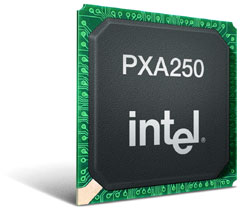
\includegraphics[scale=0.5]{images/pxa250}
\end{center}

\subsubsection{Tarjeta de expansi\'on Cerf IO 250}

	La tarjeta de expansi\'on Cerf IO 250 es una placa con entrada y salida
de propósito general. Viene equipada con un puerto serial de depuraci\'on RS232,
dos puertos seriales RS232, un puerto serial RS422/485, entre otros.

\subsubsection{Tarjeta de expansi\'on CerfComm 250}

	La tarjeta de expansi\'on CerfComm 250 est\'a equipada con caracter\'isticas
en la comunicaci\'on, viene con un controlador USB Host, un puerto Ethernet  10/100
 y tres puertos seriales de depuraci\'on RS232.

\subsubsection{Resultados}

	Para la realización de las pruebas consideramos una cantidad de datos 
igual a 50000, por otro lado programamos dos ejemplos, el primero de ellos consiste 
en la implementación mas rápida de codificar, sugerida por los papers, mientras 
que el segundo ejemplo incluye las optimizaciones sugeridas,
a continuación los resultados:\\

\begin{tabular}{|l|l|l|l|l|}
\hline
& Normal & Optimización 1 & Optimización 2 & Optimización 3 \\
\hline
Tiempo ejecución [s] & 143 & 55 & 54 & 54\\
\hline
\end{tabular}

\begin{itemize}
	\item Optimización 1: Calculo previo de funciones trigonométricas
	\item Optimización 2: Array merging
	\item Optimización 3: Blocking
\end{itemize}

